\documentclass[11pt,twoside,a4paper]{article}
% http://www-h.eng.cam.ac.uk/help/tpl/textprocessing/latex_maths+pix/node6.html symboles de math
% http://fr.wikibooks.org/wiki/Programmation_LaTeX Programmation latex (wikibook)
%=========================== En-Tete =================================
%--- Insertion de paquetages (optionnel) ---
\usepackage[french]{babel}   % pour dire que le texte est en fran{\'e}ais
\usepackage{a4}	             % pour la taille   
\usepackage[T1]{fontenc}     % pour les font postscript
\usepackage{epsfig}          % pour gerer les images

\usepackage{amsmath, amsthm} % tres bon mode mathematique
\usepackage{amsfonts,amssymb}% permet la definition des ensembles
\usepackage{float}           % pour le placement des figure
\usepackage{verbatim}

\usepackage{longtable} % pour les tableaux de plusieurs pages

\usepackage[table]{xcolor} % couleur de fond des cellules de tableaux

\usepackage{tikz}

\usepackage{lastpage}

% \usepackage[top=1.5cm, bottom=1.5cm, left=1.5cm, right=1.5cm]{geometry}
% gauche, haut, droite, bas, entete, ente2txt, pied, txt2pied
\usepackage{vmargin}
\setmarginsrb{1.0cm}{1.0cm}{1.0cm}{1.0cm}{15pt}{3pt}{60pt}{3pt}

\usepackage{lscape} % changement orientation page
%\usepackage{frbib} % enlever pour obtenir references en anglais
% --- style de page (pour les en-tete) ---
\pagestyle{headings}

% % % en-tete et pieds de page configurables : fancyhdr.sty

% http://www.trustonme.net/didactels/250.html

% http://ww3.ac-poitiers.fr/math/tex/pratique/entete/entete.htm
% http://www.ctan.org/tex-archive/macros/latex/contrib/fancyhdr/fancyhdr.pdf
\usepackage{fancyhdr}
\pagestyle{fancy}
% \newcommand{\chaptermark}[1]{\markboth{#1}{}}
% \newcommand{\sectionmark}[1]{\markright{\thesection\ #1}}
\fancyhf{}
\fancyhead[LE,RO]{\bfseries\thepage}
\fancyhead[LO]{\bfseries\rightmark}
\fancyhead[RE]{\bfseries\leftmark}
\fancyfoot[LE]{\thepage /\pageref{LastPage} \hfill
	Arcanes -- \emph{Un JdR de Tarot}
\hfill 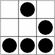
\includegraphics[width=0.5cm]{img/logo_glider.png} }
\fancyfoot[RO]{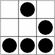
\includegraphics[width=0.5cm]{img/logo_glider.png} \hfill
	\emph{Un JdR de Tarot} -- Arcanes
\hfill \thepage /\pageref{LastPage}}
\renewcommand{\headrulewidth}{0.5pt}
\renewcommand{\footrulewidth}{0.5pt}
\addtolength{\headheight}{0.5pt}
\fancypagestyle{plain}{
	\fancyhead{}
	\renewcommand{\headrulewidth}{0pt}
}

\renewcommand{\headrulewidth}{0.25pt}
\renewcommand{\footrulewidth}{0.5pt}
%% \setlength{\headheight}{85pt}
% \addtolength{\headheight}{0.5pt}
% \fancypagestyle{plain}{
% 	\fancyhead{}
% 	\fancyfoot{}
% 	\renewcommand{\headrulewidth}{0pt}
% }

%--- Definitions de nouvelles commandes ---
\newcommand{\N}{\mathbb{N}} % les entiers naturels


%--- Pour le titre ---
\def\maketitle{%
	\begin{center}
		\begin{tabular}[c]{c|c}
			\textsc{\textbf{...}}~\\[\baselineskip]~\\[\baselineskip]
			\emph{\textbf{Version \today}}~\\[\baselineskip]~\\[\baselineskip]
			\emph{\textbf{JdR inspir{\'e} des BD \emph{Arcanes} / \emph{Arcane Majeure} / \emph{L'Histoire Secr{\`e}te}}}~\\[\baselineskip]~\\[\baselineskip]
			\textsc{Gaby Wald \& Amael Assour}~\\[\baselineskip]~\\[\baselineskip]
			& 
			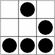
\includegraphics[width=3cm]{img/logo_glider.png}~\\[\baselineskip]
		\end{tabular}
		% \\ \hline
		 	% % if more than one logo
			% 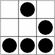
\includegraphics[width=5cm]{img/logo_glider.png}
		% \\ \hline
		% \end{tabular}
			~\\[\baselineskip]~\\[\baselineskip]
			\Huge{Arcanes}~\\[\baselineskip]
			\Large{Un JdR de tarot}~\\[\baselineskip]
		
		~\\[\baselineskip]
		~\\[\baselineskip]
	%% \large{
	%% 	\textsc{\textbf{...}}
	%% 	~\\[\baselineskip]
	%% 	<<titre personne>> : \texttt{Anne ONYME}~\\[\baselineskip]
	%% 	<<titre personne>> : \texttt{Jocelyn CONNU}~\\[\baselineskip]
	%% 	~\\[\baselineskip]
	%% 	\textit{Pr{\'e}cisions du contexte de r{\'e}daction de l'article}
	%% }

	\end{center}

}%

%--- Pour le glossaire --- a defaut de \makeglossary ou d'utilisation d'index latex

\definecolor{verylightgray}{rgb}{0.8,0.8,0.8}
\def\makeglossaire{%
	\begin{center}

	\begin{tabular}{|>{\columncolor{verylightgray}} p{0.20\textwidth}|p{0.70\textwidth}|}

		\hline

		\textbf{Carte RS} & 
			\begin{tabular}{p{0.68\textwidth}}
				Au d{\'e}but des ann{\'e}es 80, on trouva un catalyseur de l'effet RS en l'esp{\`e}ce de curieuses cartes, dont on ignore {\`a} peu pr{\`e}s tout. les premi{\`e}res cartes firent leur apparition dans la r{\'e}gion de Seattle, USA. On cherche encore {\`a} percer l'identit{\'e} du ou des cr{\'e}ateurs des premiers paquets. 
				La C.I.A., comprenant rapidement l'immense potentiel tactique que recelaient les cartes, cr{\'e}a Stargate, un groupe de scientifiques charg{\'e} d'anakyser le ph{\'e}nom{\`e}ne et de former des agents capables de le contr{\^o}ler : les agents RS.
			 \end{tabular} \\
		\hline
		\textbf{Agent RS} & 
			\begin{tabular}{p{0.68\textwidth}}
				D{\`e}s le d{\'e}but, les premiers agents RS remport{\`e}rent des succ{\`e}s impresionnants, accomplissant des missions alors que toutes les chances de r{\'e}ussites {\'e}taient contre eux. 
				Les diff{\'e}rentes op{\'e}rations Stargate sont encore class{\'e}es "secret d{\'e}fense" mais les chercheurs pointent le doigt sur un certain nombre d'{\'e}v{\`e}nements, comme la mort du Pr{\'e}sident panam{\'e}en en 82 ou le putsch rat{\'e} des g{\'e}n{\'e}raux russes. 
				Certains affirment que les cartes existent de toute {\'e}ternit{\'e}, et que nos cartes {\`a} jouer en seraient des formes simplifi{\'e}es. 
			\end{tabular} \\
		\hline
		\textbf{Grade Stargate} & 
			\begin{tabular}{p{0.68\textwidth}}
				On a pris l'habitude de classer les agents Stargate {\`a} partir des figures des cartes {\`a} jouer classiques : 6, 8, 9, 10, Valet, Cavalier, etc. Ainsi, un 6 n'est sans doute capable que d'influer sur de petits {\'e}v{\`e}nements ayant peu de possibilit{\'e}s statistiques, comme le lancement d'une pi{\`e}ce de monnaie par exemple. Les grades sup{\'e}rieurs peuvent agir beaucoup plus en profondeur sur la trame du hasard.
			\end{tabular} \\
		\hline
%% 		\textbf{DEA (Drug Enforcement Administration)} & 
%% 			\begin{tabular}{p{0.68\textwidth}}
%% 				Agence gouvernementale am{\'e}ricaine charg{\'e}e de la lutte anti-drogue dans le monde.
%% 			\end{tabular} \\
%% 		\hline  
%% 		\textbf{Nagual} & 
%% 			\begin{tabular}{p{0.68\textwidth}}
%% 				Esprit, double de l'esprit humain.
%% 			\end{tabular} \\
%% 		\hline 
		\textbf{Comit{\'e} Magic} & 
			\begin{tabular}{p{0.68\textwidth}}
				Organisme Ultra-secret mis en place par les Alli{\'e}s durant la Seconde Guerre Mondiale pour {\'e}tudier, utiliser les cartes et manipuler le hasard. Il n'avait de compte {\`a} rendre qu'{\`a} Churchill et Roosevelt. Magic fut dissous en 1946. 
				Magic travailla en {\'e}troite collaboration avec Ultra, le programma de d{\'e}codage des messages secrets allemands [Enigma] puis avec Manhattan, le programme de r{\'e}alisation de la premi{\`e}re bombe atomique am{\'e}ricaine {\`a} Los Alamos. 
				Les bras arm{\'e}s de Magic {\'e}taient, du c{\^o}t{\'e} anglais : le SOE (Special Operation Executive), et c{\^o}t{\'e} am{\'e}ricain l'OSS (anc{\^e}tre de la CIA), comme Magic, ces deux entit{\'e}s furent dissoutes au lendemain de la guerre, du moins officiellement.
			\end{tabular} \\
		\hline 
		\textbf{Fondation Vane} & 
			\begin{tabular}{p{0.68\textwidth}}
				Agence gouvernementale am{\'e}ricaine qui prit la suite de Magic. Les anglais refus{\`e}rent d'en faire partie. Au d{\'e}part, il s'agissait d'un simple programme d{\'e}tude des ph{\'e}nom{\`e}nes RS.
			\end{tabular} \\
		\hline 
		\textbf{Stargate} & 
			\begin{tabular}{p{0.68\textwidth}}
				Successeur de la Fondation Vane dans les ann{\'e}es 60. Dot{\'e} d'un budget beaucoup plus important, et plus tourn{\'e} vers l'utilisation des cartes que vers leur {\'e}tude.
				Programme de la C.I.A. qui cherche depuis plusieurs ann{\'e}es {\`a} percer le secret des cartes RS et qui, dans le m{\^e}me temps, les utilise pour former des agents RS capables de manipuler le hasard. Ces agents, tr{\`e}s rares et tr{\`e}s fragiles psychologiquement ont un immense potentiel tactique. Ils peuvent, {\`a} la lettre, accomplir des miracles, gagner contre toutes les probailit{\'e}s, mlais qui sont-ils vraiment, et en derni{\`e}re analyse, qui les contr{\^o}le ?
			\end{tabular} \\
		\hline 
		\textbf{R{\'e}tro-Synchronicit{\'e} (RS)} & 
			\begin{tabular}{p{0.68\textwidth}}
				Th{\'e}orie selon laquelle le hasard n'existe pas. Elle suppose qu'on peut orienter les {\'e}v{\`e}nements et le futur {\`a} condition de disposer d'un catalyseur qui d{\'e}clenche et acc{\'e}l{\`e}re la r{\'e}action. ces catalyseurs seraient en l'occurrence des cartes qui seraient les anc{\^e}tres de nos jeux de cartes.
			\end{tabular} \\
		\hline
		\textbf{Singularit{\'e} ou effet RS} & 
			\begin{tabular}{p{0.68\textwidth}}
				Moment o{\`u} l'action des cartes se d{\'e}clenche. Le sujet est alors devant les possibilit{\'e}s offertes par le futur, {\`a} lui de choisir les plus int{\'e}ressantes. Plus une singularit{\'e} est profonde, plus les possibilit{\'e}s sont nombreuses et plongent plus loin dans le futur. 
			\end{tabular} \\
		\hline

	\end{tabular}

\end{center}

}%

%============================= Corps =================================
\begin{document}
%ecrire le titre...
\maketitle
\setcounter{page}{0}
\thispagestyle{empty}
\clearpage

\setcounter{page}{0}
\thispagestyle{empty}

~\\

\clearpage
\setcounter{page}{0}
\thispagestyle{empty}
% ecrire la table des mati{\'e}res...
\tableofcontents

% \clearpage

% \setcounter{page}{0}
% \thispagestyle{empty}

% ecrire la table des figures et celle des tableaux

%% \setcounter{page}{0}
%% \thispagestyle{empty}
%% ~\\ \rule{10cm}{1mm}~\\
%% \listoffigures
%% ~\\ \rule{10cm}{1mm}~\\
%% \listoftables
\clearpage

\setcounter{page}{1}

\section*{Introduction\markboth{Introduction}{Introduction}}

\addcontentsline{toc}{section}{Introduction}


[...]~\\

\rule{10cm}{0.5mm}~\\


\clearpage

\section{{\'E}l{\'e}ments de base, id{\'e}es...}

\subsection{R{\^o}le des cartes}

{ \setlength\parindent{0pt} \small
\begin{tabular}[c]{c c c c c c}
	\rowcolor{verylightgray}
	Famille			&	Symbole			&	{\'E}l{\'e}ment	& 	Type / Groupe... ou Id{\'e}al (?)		& Famille "CyberPunk" (?)		& "Pouvoirs"			\\
	Arcanes			&	Nb et Nom		&	-- selon --		&	Magie (?) ...							& Magie (?) ; Hasard ... 		& ... 					\\
	Bâtons			&	Carreaux		&	Air				&	Sociabilit{\'e}, Charisme ; Sant{\'e}	& Gangs, Nomades...				& Social / Relation 	\\
	Coupes			&	C\oe ur			&	Eau				& 	Vie, Gu{\'e}rison ; Ing{\'e}nierie		& Tech, MedTech... 				& Mat{\'e}riel			\\
	Deniers			&	Piques			&	Terre			& 	Protection, R{\'e}flexion ; Fortune		& Solos, Fixers, Hackers...		& Virtuel / Intellect	\\
	{\'E}p{\'e}es	&	Tr{\`e}fles		&	Feu				& 	Pouvoir, Unification ; Action			& Corporations, {\'E}tats...	& Temporel / Religieux	\\
	
	%% Erlin => Deniers => Trèfles
	%% Dyo => Coupes => Coeurs
	%% Reka => Bâtons => Piques
	%% Aker => Épées => Carreaux
\end{tabular} }~\\

Tirage des PJ : 5 {\`a} 10 cartes classiques ; d{\'e}termination puissance dans chaque caract{\'e}ristique, si t{\^e}te : cela permet de d{\'e}terminer une appartenance {\`a} une maison (ou deux ?) et un niveau au sein ce celle(s)-ci. ~\\

Pendant une partie : un jeu de tarot complet (une campagne ?) ou un jeu classique de 54 cartes (ou deux, selon les besoins ou la variante utilis{\'e}e), symbolisant jeu(x) construit(s) "dans le jeu" (intra-di{\'e}g{\'e}tique) "{\`a} la demande", ou apparus voire d{\'e}couverts selon les circonstances... ~\\

\subsection{R{\'e}solution des actions des PJ / Phase d'Action}

Rappel / R{\`e}gle d'or : une action triviale r{\'e}ussit toujours !~\\

Initiative par tirage d'une carte dans un jeu sp{\'e}cifique m{\'e}lang{\'e} ({\`a} moins que le premier intervenant ne prenne les autres par surprise) : cela peut {\^e}tre dans la pile de cartes restantes, une r{\'e}serve de cartes du MJ.~\\

Chaque joueur dispose d'une main de cinq (5) cartes, renouvelable au fur et {\`a} mesure de son utilisation apr{\`e}s chaque usage d'une ou pluseurs cartes dans une pile de tirage d{\'e}di{\'e}e, en compl{\'e}tion {\`a} 5 (sauf sp{\'e}cificit{\'e}s).~\\
Une action se r{\'e}sout par le d{\'e}p{\^o}t d'une ou plusieurs cartes par chaque joueur pour son PJ, le d{\'e}compte du "score" s'effectue de la fa\c{c}on suivante (hors Atouts / Arcanes) : 
\begin{itemize}
	\item Valeur faciale des cartes li{\'e}es au type ou au groupe utilis{\'e} (de l'as qui vaut 1 au 14 pour la plus haute t{\^e}te) ; 
	\item Un demi point par autres cartes non li{\'e}es au type ou au groupe utilis{\'e} ; 
	\item Un Joker (ou Excuse) vaut toujours 7 ; 
	\item Dans les combinaisons sp{\'e}ciales (paire, brelan, suite...), multipliez le score pr{\'e}c{\'e}demment obtenu par le nombre de cartes de la combinatoire ; 
	\item \emph{Optionnel : }Un Atout ou une Arcane (ou un Joker) permet une action sp{\'e}ciale (contr{\'e} par un Atout de valeur sup{\'e}rieure) : 
	\begin{itemize}
		\item Tirage de cartes suppl{\'e}mentaires (valeur de l'Atout divis{\'e} par trois (3), arrondi au sup{\'e}rieur ; ou 1d6) ; 
		\item Rejouer imm{\'e}diatement (apr{\`e}s compl{\'e}tion de la main) ; 
		\item Action h{\'e}ro{\"i}que (dont la r{\'e}ussite d{\'e}pend du reste des cartes jou{\'e}es avec celle-ci). 
	\end{itemize}
	\item \emph{Optionnel : }Utilisation d'une Carte Sp{\'e}ciale d{\'e}finissant le PJ : {\`a} d{\'e}finir {\`a} l'avance entre le MJ et le joueur (valeur de la carte), mise en jeu de la vie du PJ et : ou du pouvoir associ{\'e} {\`a} cette carte. 
\end{itemize} %% ~\\

Les cartes jou{\'e}es rejoignent une d{\'e}fausse en attendant d'{\^e}tre rem{\'e}lang{\'e}es pour cr{\'e}er une nouvelle pile de tirage quand celle-ci est vide.~\\

\clearpage 

En dehors d'un Phase d'Action, on peut utiliser un "Effet R{\'e}troSynchronicit{\'e}" (RS) : un joueur pose une carte sur la table en pr{\'e}vision d'une utilisation future (avec une annotation ou un post-it) ; cela permet d'avoir un {\'e}l{\'e}ment utile par la suite et que le joueur peut ainsi faire appara{\^i}tre par la suite (v{\'e}hicule, {\'e}l{\'e}ment de d{\'e}cor...). Cette carte est ensuite int{\'e}gr{\'e}e {\`a} la pile de tirage : quand cette carte est tir{\'e}e, elle est forc{\'e}ment en faveur du joueur l'ayant d{\'e}pos{\'e}e (int{\'e}gration {\`a} sa main courante). Cela peut {\^e}tre utile selon puissance et typologie de la carte concern{\'e}e, et l'objet concern{\'e}.~\\

\subsection{Ressorts pour le MJ}

Quelques {\'e}l{\'e}ments {\`a} utiliser par le MJ comme ressorts d'action, {\`a} communiquer ou {\`a} faire d{\'e}couvrir : 
\begin{itemize}
	\item Les cartes, leurs utilisations et les porteurs de cartes sont rep{\'e}rables {\`a} distance par d'autres (adversaires ou non) : bruit blanc / color{\'e} perceptible, cartes qui chauffent (pour les joueurs)... ; 
	\item Certains mat{\'e}riaux peuvent servir d'isolants : eau, tissus (soie ou autres mat{\'e}riaux sp{\'e}cifiques)...
	\item Il est possible de marquer des lieux par des glyphes, de m{\^e}me pour les gens (tatouages) ou certains objets : cela peut servir de protection, dans un sens comme dans l'autre (bloquer {\`a} l'int{\'e}rieur ou {\`a} l'ext{\'e}rieur) ; 
	\item Lois physiques modifiées en certains lieux (géométrie non euclidienne : on entre dans un bâtiment, la sortie abouti ailleurs...) ; 
	\item ... 
\end{itemize}~\\

\subsection{Variantes et modes de jeu (jeu en campagne)}

Ces variantes peuvent compl{\'e}ter ou remplacer les r{\`e}gles d{\'e}crites pr{\'e}c{\'e}dentes.~\\

Variante (jeu en campagne) : chaque joueur dispose au d{\'e}part de la campagne d'un jeu complet (54 ou 78 cartes) et peut utiliser ses cartes comme bon lui semble ; les cartes tir{\'e}es pour d{\'e}finir son personnage sont consid{\'e}r{\'e}es comme maitresses et peuvent n'{\^e}tre actives qu'en certaines circonstances.~\\

Destructions de cartes ? Annotations sp{\'e}cifiques ? Par exemple les cartes du tirage du personnage du joueur ou tir{\'e}es pendant la partie ; si n{\'e}cessaire on subtitue par un carton solide (carte bristol) avec annotations.~\\

\subsection{Modalit{\'e}s particuli{\`e}res}

Modalit{\'e}s CyberPunk : magie limit{\'e} au monde virtuel (matrice / cyberespace) et classiquement reli{\'e} {\`a} la mythologie vaudoue (at autres {\'e}l{\'e}ments cultures Cara{\"i}bes). 
Relier {\`a} une autre mythologie dans un autre univers (de jeu) : romain, grec, sum{\'e}rien, {\'e}gyptien, nordique, inca... (NOTE : tableau de correspondances {\`a} faire !)

\subsection{Symboles et design / dessin des cartes}

N'importe quel jeu de cartes ou de tarot peut faire l'affaire ; ceux à petit prix peuvent faire l'affaire (selon le mode de jeu), ou de votre propre dessin. L'essentiel est de pouvoir les utiliser facilement pendant la ou les parties.~\\

\begin{minipage}[ht]{0.45\textwidth}
	FEU / AIR / EAU / TERRE
\end{minipage} \hfill \begin{minipage}[ht]{0.45\textwidth}
	\def\triangle{--++(120:1)--++(240:1)--cycle}
	\def\triangleReverse{--++(240:1)--cycle}
	\begin{tikzpicture}
		\tikz\draw[red,thick](0,0)\triangle; %% FEU
		
		\tikz\draw[blue,thick](2,0)\triangle (1,0.40)--(2,0.40); %% AIR
		
		\tikz\draw[orange,thick](3,1)--(4,1)\triangleReverse; %% EAU
		
		\tikz\draw[green,thick](5,1)--(6,1)\triangleReverse (5,0.60)--(6,0.60); %% TERRE
	\end{tikzpicture}
\end{minipage}

%% utilisation packages latex tikz / tikzpeople pour figures et dessins de fonds
%% tikz-3dplot ?
%% tikzsymbols ?
%% tikz-network ?
%% ... 
%% find /usr/share/ -name "tikz*"
%% find /usr/share/tex* -name "*card*"
%% find /usr/share/tex* -name "*game*"
%% find /usr/share/tex* -name "*chess*"
%% %% /usr/share/texlive/texmf-dist/tex/generic/pgf/frontendlayer/tikz/libraries/tikzlibraryshapes.symbols.code.tex
%% chercher dans : 
%% %% /usr/share/doc/texlive-doc/latex
%% %% /usr/share/texlive/texmf-dist/makeindex/latex
%% %% /usr/share/texlive/texmf-dist/source/latex
%% %% /usr/share/texlive/texmf-dist/tex4ht/ht-fonts/alias/latex
%% %% /usr/share/texlive/texmf-dist/tex4ht/ht-fonts/unicode/latex
%% %% /usr/share/texlive/texmf-dist/tex/latex
%% %% /usr/share/texmf/doc/latex
%% %% /usr/share/texmf/tex/latex


\clearpage


%% \section{Section}
%% \subsection{Sous-section}
%% \subsubsection{sous sous sous section}
%% [...]~\\
%% \subsubsection{sous sous sous section}
%% \subsection*{SousSectionNonNumerot}
%% \addcontentsline{toc}{section}{SousSectionNonNumerot}
%% \begin{table}[ht]
	%% \begin{center}
		%% \begin{tabular}{|p{0.1\textwidth}|p{0.7\textwidth}|}
		%% \hline
		%% 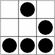
\includegraphics[width=1cm]{img/logo_glider.png}
		%% & 
		%% \textbf{GLIDER} est le logo des hacker, symbole repris du jeu de la vie (cavalier). \\
		%% \hline
		%% \end{tabular}
	%% \end{center}
	%% \caption{Un tableau r{\'e}f{\'e}renc{\'e}}
	%% \label{tab:TabReference01}
%% \end{table}~\\
%% \clearpage
%% \subsection{Encore une sous-section}
%% \begin{figure}[H]
	%% \centerline {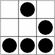
\epsfig {file=img/logo_glider.png,width=0.5\textwidth}}
	%% \caption{Une belle image}
	%% \label{fig:FigReference01}
%% \end{figure}
%% \clearpage

\section{Annexes}

\subsection{Glossaire}

%% voir en haut : sous la definition du titre : glossaire

\makeglossaire

\clearpage

\subsection{Jeu de r{\^o}le g{\'e}n{\'e}rique de Philippe Tromeur : Arcanes}

Source : \texttt{http://philippe.tromeur.free.fr/53/arcanes.pdf}, publi{\'e} le mardi 10 juin 2008.

\subsubsection{Le mat{\'e}riel et les personnages}

Ce jeu de r{\^o}le se joue avec un jeu de tarots normal, mais vous pouvez {\'e}galement utiliser un jeu de tarot divinatoire, si \c{c}a vous amuse.
Durant la partie, chaque joueur a une main de cinq cartes, renouvell{\'e}es au fur et {\`a} mesure du jeu. Les autres cartes sont dispos{\'e}es dans une pioche tourn{\'e}e contre la table.
Papier, crayons et victuailles sont utiles...~\\

Les personnages sont d{\'e}finis par 5 Couleurs not{\'e}es A, B, C, D et E : Arcane, B{\^a}tons, Coupes, Deniers et {\'E}p{\'e}es.
Le joueur peut r{\'e}partir 22 points entre ses 5 caract{\'e}ristiques, sachant que l'Arcane co{\^u}te deux fois plus cher que les autres Couleurs. 
Pour chaque Couleur, choisir une sp{\'e}cialit{\'e}. ~\\

\begin{minipage}[ht]{0.40\textwidth}

	\subsubsection{Tirage de cartes}
	
	Pour effectuer une action, utilisez une carte de votre main ou tirez-en une de la pioche.
	Chaque action est associ{\'e}e {\`a} une Couleur :
	\begin{itemize}
		\item[Arcanes] (ou Atouts) pour la magie
		\item[B{\^a}tons] (ou Carreau) pour la sant{\'e}
		\item[Coupes] (ou Coeurs) pour le charme
		\item[Deniers] (ou Tr{\`e}fles) pour la fortune
		\item[Ep{\'e}es] (ou Pique) pour l'action
	\end{itemize}

\end{minipage} \hfill \begin{minipage}[ht]{0.54\textwidth}

	\subsubsection{Personnages joueurs (PJ) et Personnages non joueurs (PNJ)}
	
	Le R{\'e}sultat est la valeur de la carte pos{\'e}e, ajout{\'e}e au score du personnage dans la Couleur de l'action. Si la carte est de la Couleur de l'action, le score du personnage compte double.
	L'Excuse / le Mat compte pour 0 ; les Valets 11, les Cavaliers 12, les Dames 13, les Rois 14. 
	Par exemple : un personnage chante, avec un score de 5 en Coeur. Il pose le Valet de Coeur : le R{\'e}sultat est donc de (5x2)+11=21

\end{minipage}~\\

Le ma{\^i}tre du jeu a une seule main utilis{\'e}e pour l'ensemble des personnages non joueurs.

\subsubsection{Combat}

Un combat consiste en des oppositions en Ep{\'e}e : le vainqueur a bless{\'e} l'adversaire. Ce dernier doit faire une opposition contre une difficult{\'e} d{\'e}pendant de l'arme (et souvent du score de B{\^a}tons de l'attaquant) :~\\
\begin{tabular}[c]{c c c c}
	Poings		&	2xB{\^a}tons	&	Pistolet		&	20	\\
	Couteau		&	5+B{\^a}tons	&	Fusil			&	30	\\
	Ep{\'e}e	&	10+B{\^a}tons	&	Lance-Pierre	& 	5	\\
\end{tabular}~\\
En cas d'{\'e}chec (r{\'e}sultat inf{\'e}rieur {\`a} la difficult{\'e}), c'est une blessure grave, sinon c'est une blessure l{\'e}g{\`e}re. En cas d'{\'e}chec critique (r{\'e}sul tat inf{\'e}rieur {\`a} la moiti{\'e} de la difficult{\'e}), c'est une blessure critique (et le coma).
Avec une blessure l{\'e}g{\`e}re, on n'a plus que 3 cartes en main. Avec une blessure grave, on n'en a plus qu'une en main. On r{\'e}cup{\`e}re un niveau de blessure par jour de soins appropri{\'e}s.

\subsubsection{Sp{\'e}cialit{\'e}s et Magie, Exp{\'e}rience, Aventure... }

Les sp{\'e}cialit{\'e}s autorisent les personnages {\`a} rajouter +5 {\`a} leur R{\'e}sultat, si jamais l'action est li{\'e}e au champ de cette sp{\'e}cialit{\'e}. Pour utiliser la magie, il faut poss{\'e}der la sp{\'e}cialit{\'e} ad{\'e}quate :
\begin{itemize}
	\item[] n{\'e}cromancie pour discuter avec des fant{\^o}mes,
	\item[] d{\'e}monisme pour appeler des d{\'e}mons,
	\item[] divination pour savoir des choses,
	\item[] t{\'e}l{\'e}kin{\'e}sie pour d{\'e}placer des objets...
\end{itemize}
La difficult{\'e} d'Arcane, incluant le bonus de +5 pour la sp{\'e}cialit{\'e}, est g{\'e}n{\'e}ralement {\'e}lev{\'e}e, de 20 pour une divination mineure, {\`a} 40 pour la destruction d'un immeuble par la foudre.
Plusieurs tentatives successives sont possibles, mais en cas d'{\'e}chec critique (R{\'e}sultat inf{\'e}rieur {\`a} la moiti{\'e} de la difficult{\'e}), le r{\'e}sultat est catastrophique, par exemple une blessure.
En prenant son temps (une heure par jet d'Arcane), on {\'e}vite le risque d'{\'e}chec critique.~\\

Apr{\`e}s une aventure, un personnage gagne de 1 {\`a} 5 points d'exp{\'e}rience, qui se d{\'e}pensent pour acheter de nouveaux points dans les 5 Couleurs (l'Arcane co{\^u}te toujours deux fois plus cher). Une sp{\'e}cialit{\'e} co{\^u}te 3 points, sauf les sp{\'e}cialit{\'e}s Arcanes qui co{\^u}tent 5 points. 
--- Oup's, nous arrivons d{\'e}j{\`a} en fin de page et je n'ai pas l'espace de vous pr{\'e}senter un univers et un exemple de sc{\'e}nario... D{\'e}brouillez-vous, je vous fais confiance !

\clearpage

\subsection{Autres JdR / Jeux de R{\^o}le utilisant un Tarot}

\begin{itemize}
	\item \emph{Les Lames du Cardinal} (Tarot des Ombres) ; 
	\item Tarot d'inspiration pour \emph{R{\^e}ves de Dragon}, \emph{Mal{\'e}fices}
	\item \emph{Ambre}, \emph{Mage}...
	\item ...
	\item Cas {\`a} part et m{\'e}ritant d'{\^e}tre cit{\'e} ici : \emph{Ch{\^a}teau FalkenStein}, o{\`u} plusieurs jeux de 54 cartes sont utilis{\'e}s {\`a} la place des d{\'e}s en cours de partie afin de r{\'e}soudre les actions des personnages de joueurs.
\end{itemize}

\subsection{Bibliographie\markboth{Bibliographie}{Bibliographie}}

\addcontentsline{toc}{section}{Bibliographie}
\nocite{*}
%toutes references biblio : 6 lettres + 2 chiffres
\bibliography{arcanesJdR}
\bibliographystyle{frplain} % plain or frplain
\end{document}
